\begin{otherlanguage}{swedish}

    \newcommand{\name}{Svensk sammanfattning}
    \chapter*{\name{}\\\large{Subjektiva taggar vid personlig kategorisering av ljud}}
    \addcontentsline{toc}{chapter}{\name}

    \section*{Inledning}
    Människor intar dagligen en stor dos av ljud i dagens värld. Större helheter av ljud byggs upp med ljudeffekter, jinglar, loopar och andra ljudfragment. Tillsammans används de för att skapa ljudlandskap avsedda för olika ändamål. Skapandeprocessen och förfaringssättet bakom alla de här ljuden är mindre påtagligt i vardagen och få är helt insatta i hur ljuden blir till.

    Yrket som ljuddesigner innebär att skapa och hantera ljud avsedda för ett visst ändamål eller en viss produkt. Arbetet förutsätter mycket kreativitet och fantasi för att få fram de ljud som situationen kräver. Verktygen som ljuddesigner använder sig av för att hantera ljud måste vara så lätta som möjligt att förstå för att arbetsprocessen ska kännas inspirerande och effektiv. Annars kan det uppstå frustrerande situationer där motivationen lätt försvinner.

    I huvudsak finns det två olika tillvägagångssätt för att skapa ljud ämnade för film, spel och andra medier. Det första alternativet är att skapa alla ljud från grunden genom att spela in dem i en studio med lämplig utrustning. Man har då möjlighet att utforma exakt sådana ljud man vill ha, men processen kan bli både dyr och tidskrävande eftersom flera ljud ofta behövs för att tillsammans kombineras till ett tillfredsställande resultat.

    Den andra varianten, som är i fokus i den här avhandlingen, är att använda sig av befintliga ljudbibliotek med färdigt inspelade och kategoriserade ljud. Biblioteken kan innehålla ett fåtal eller flera tusen ljud, där likheten mellan ljuden varierar. Problemet med det här alternativet är att det inte finns en etablerad standard för hur ljuden ska indelas och klassificeras. Indelningarna är vanligen gjorda manuellt med olika former av konkreta taggar som redogör för ljudkällan, vad som händer i ljudklippet, eller liknande beskrivningar. En rad sökverktyg finns tillgängliga för att hitta ljud bland ljudbiblioteken, men på grund av variationen mellan de olika samlingarnas kategoriseringssystem blir sökningsresultatet ofta mediokert.

    En genomgående brist i sökverktygen och ljudbibliotekens kategoriseringssystem är att de inte tar subjektivitet i beaktande. Människor beskriver ofta ljud i subjektiva ord, vilket tyder på att personliga taggar skulle kunna vara till stor hjälp för att klassificera och hantera ljud. Problemet med att implementera subjektiva taggar i ett kategoriseringssystem är att de är individuella; samma ljud kan ha olika beskrivningar beroende på vem man frågar. Processen att förse ljud med subjektiva beskrivningar borde således göras skilt för varje användare, men att manuellt tagga ljud är både tidskrävande, arbetsdrygt och felbenäget.

    \section*{Mål}
    Målet med den här avhandlingen är att ta fram ett lösningsförslag på hur subjektivitet kan implementeras i sökverktyg ämnade för ljudbibliotek. Lösningsförslaget som utvecklats är ett fungerande program, men tjänar mera som ett utkast till hur kategorisering med subjektiva beskrivningar kan se ut. Programmet ger användare möjligheten att med sina egna subjektiva ljudupplevelser kategorisera ljud genom att märka dem med subjektiva taggar. Varje användare kan alltså klassificera ljud enligt eget tycke och smak. För att underlätta det manuella arbetet som krävs söks liknande ljud automatiskt upp med hjälp av maskininlärning och taggas enligt en användares preferenser.

    Avsikten med att inkorporera subjektivitet i sökverktygen är att underlätta det dagliga arbetet som exempelvis en ljuddesigner gör genom att erbjuda ett alternativt sätt att organisera och söka fram ljud. Inkorporeras lösningsförslaget vidare och utvecklas till en färdig produkt kan helheter av ljud förhoppningsvis byggas upp på ett bättre och smidigare sätt, vilket därmed också sparar tid och pengar för de som anställer ljuddesigners.

    \newpage\section*{Tillämpning}
    \begin{figure}[ht]
        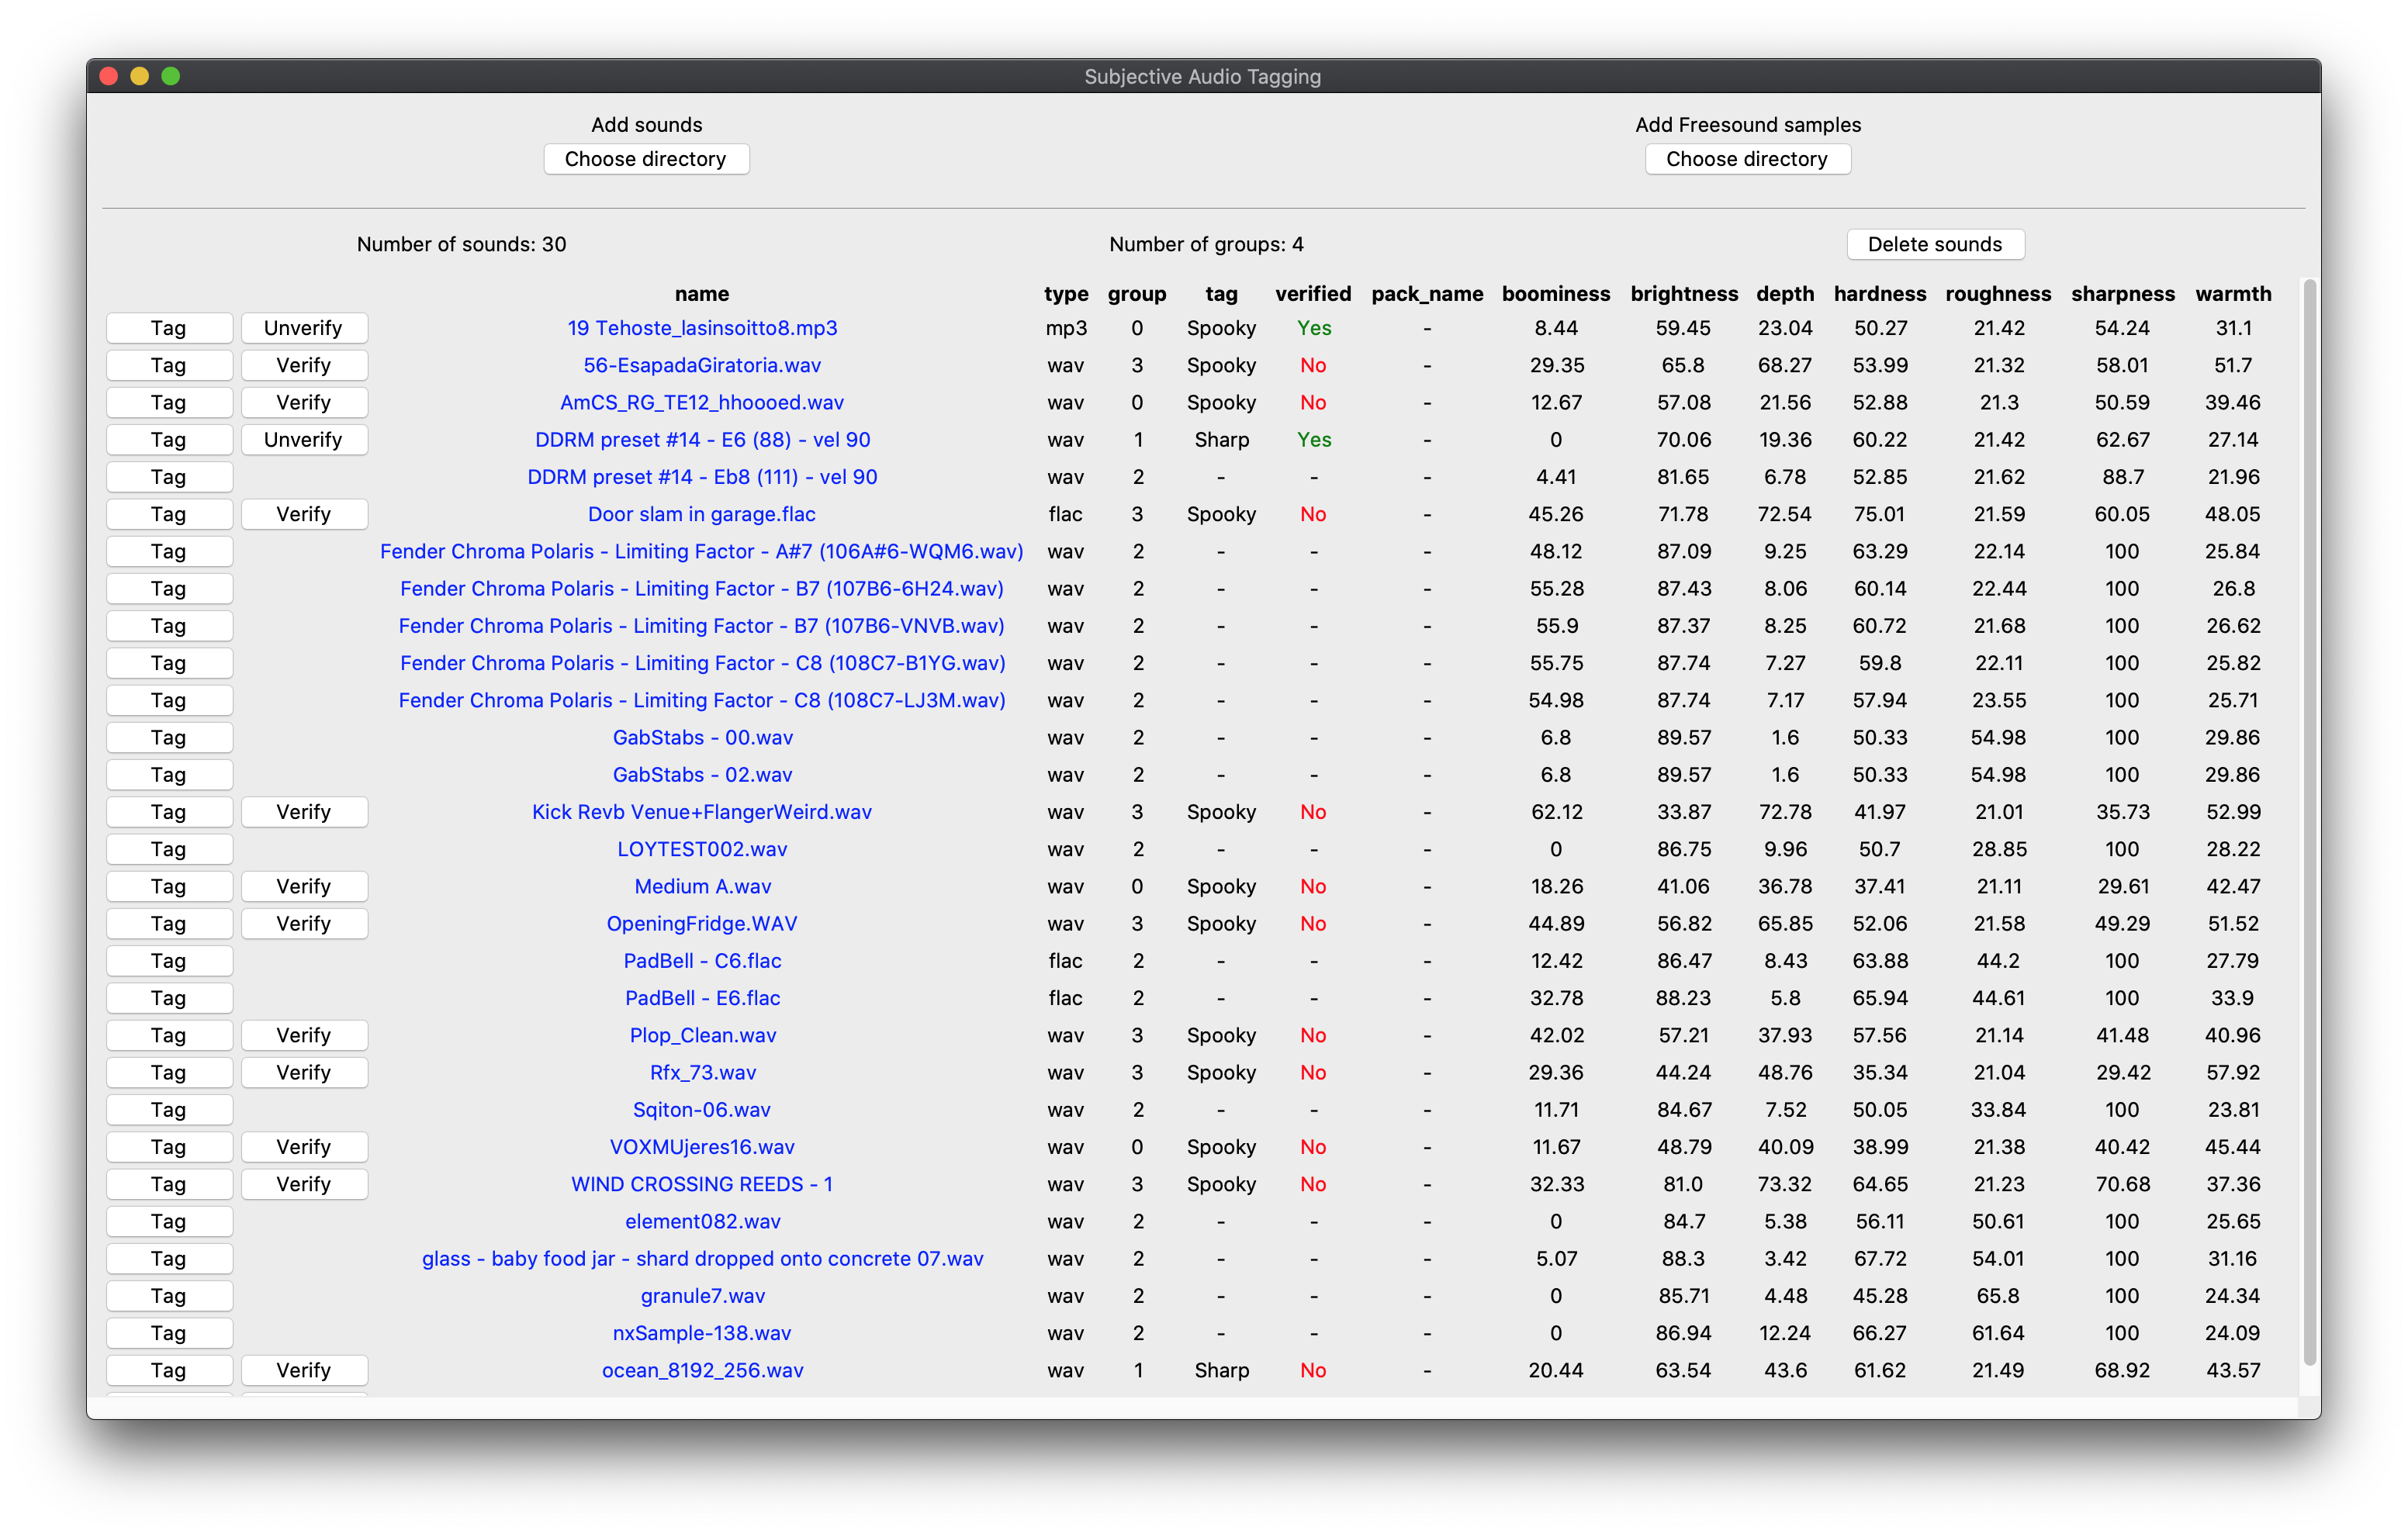
\includegraphics[width=\textwidth]{figures/app/ui}
        \caption{Bild på det utvecklade programmet i användning.}\label{bild}
    \end{figure}

    Som lösningsförslag till de nämnda problemen med subjektivitet vid ljudklassificering beskrivs ett utvecklat program som är kapabelt att justera sig enligt en användare. Programmet är gjort i Python och syftet är att demonstrera hur man kan minska det manuella arbete som krävs för att kategorisera ljud efter de preferenser och ljuduppfattningar varje enskild användare har. Upplägget och designen kan ses i \cref{bild}. Valda ljud som läggs till i programmet analyseras och grupperas, varefter de sparas i en databas och visas upp i en tabell där användaren kan tagga och verifiera ljuden. Viktigt att notera är att endast en beskrivning kan ges åt varje ljud. Ett ljud kan exempelvis inte ha både taggen ”skrämmande” och ”lugnande”, men ljud i olika grupper kan dela samma definition; två grupper av ljud kan alltså båda ha beskrivningen ”värmande”.

    Kärnan i programmet som hjälper användaren med kategoriseringen är ett automatiskt klassificeringssystem som utformats med hjälp av maskininlärning. Systemet delar internt in liknande ljud i grupper baserat på deras klangfärg, eller timbre, genom att analysera ljuden med biblioteket timbral\_models. Ljuden processeras och får sju stycken tillhörande numeriska värden utmärkta, som varierar från 0 till 100. De här värdena används i sin tur när programmet söker efter motsvarande ljud; ju fler värden som ligger nära varandra mellan två ljud, desto mer påminner ljuden om varandra.

    Logiken som grupperar in ljuden enligt relevans är uppbyggd av två olika maskininlärningsalgoritmer som sekventiellt får fram en inledande och en justerbar lösning. Båda algoritmerna är av typen icke-väglett lärande (unsupervised learning) och är tagna ur scikit-learn-biblioteket. Den första metoden som uppskattar hur många grupper det finns i en samling av ljud är gjord med Mean shift-algoritmen. Den söker fram naturligt förekommande grupper av data baserade på de attribut den får inmatade, i det här fallet de uträknade värdena på klangfärg. Summan som det resulterar i och som produceras är en estimerad utgångspunkt för hur många grupper det kommer att finnas i slutet när användaren kategoriserat klart.

    Den andra metoden är K-means-algoritmen som används för att kontinuerligt uppdatera grupperingarna i enlighet med hur användaren använder programmet. Till en början fungerar uppdelningarna som gjorts av Mean shift-algoritmen som startpunkt, men allteftersom användaren gör flera kategoriseringar kan det behövas nya indelningar och omorganisering i de existerande grupperna. Antalet grupper med liknande ljud kan aldrig minska, endast öka i antal – förutom när nya ljud läggs till. Den övre gränsen för antalet grupper är lika många som det finns ljud i programmet. Om en användare vill ge en specifik benämning till vart och ett av de inkluderade ljuden är det således möjligt.

    När ljud blivit tillagda, analyserade och grupperade av maskininlärningsalgoritmerna kan de bli tilldelade taggar – en singulär beskrivning per ljud – definierade av antingen användaren själv eller automatiskt av programmet. Kategoriseringar som görs av användaren antas alltid vara korrekta. Taggar som programmet automatiskt tilldelar ljud förblir obekräftade till en början, då de kan vara inkorrekta. Det här beror på att programmet inte kan vara säkert på att klassificeringarna är rätt och är sålunda pessimistiskt i sitt handlingssätt. För att hålla reda på de här två möjligheterna har varje ljud en associerad boolesk datatyp, med benämningen verified, som klarlägger om den givna taggen ett ljud har är korrekt eller inte. Programmatiskt taggade ljud kan verifieras av användaren om hen anser att de är korrekta. Verifieringen kan också återställas och ändras för vart och ett av de redan kategoriserade ljuden när som helst under användning, vilket är behändigt om man av misstag verifierat ett ljud.

    Verified-värdet bestämmer också hur programmet ska gå till väga när motsvarande ljud ska taggas. Om ett ljud klassificeras när alla ljud i dess grupp är overifierade – till exempel i början när inga ljud ännu har blivit kategoriserade – eller om ett verifierat ljud taggas om, hålls de fastlagda grupperingarna intakta. Då kommer alla ljud som tillhör samma grupp bli tilldelade den benämning som gavs till det interagerade ljudet. Det här scenariot är i princip detsamma som att döpa om taggen som hör ihop med gruppen.

    Det andra händelseförloppet inträffar när användaren väljer att kategorisera om ljud som programmet redan taggat. Då bildas och modifieras grupper ända tills ett resultat nåtts där grupperingarna överensstämmer med de kategoriseringar som användaren begär. Den tilldelade gruppen kan ändras för alla ljud, med ljud som redan är verifierade kommer behålla sina taggar. Overifierade ljud kan å andra sidan bli märkta med en ny potentiell benämning, även om de tillhör en annan grupp än det korrigerade ljudet.

    När ytterliga ljud läggs till i programmet behövs logik som ser till att de framsteg användaren redan gjort i klassificeringar bibehålls. Eftersom de nya ljuden kan befinna sig var som helst i relation till de som redan är inkluderade, kommer all gruppering att göras om och programmet applicerar alla de definierade taggarna på nytt. I och med det här kan antalet grupper ändra, men allt som användaren åstadkommit förblir oförändrat. De nyinlagda ljuden har möjligen fått en automatiskt genererad tagg om de påminner om något av de existerande ljuden.

    \subsection*{Evaluering}
    För att evaluera det utvecklade programmet används fyra konstruerade exempelfall som påvisar fungerande, men också bristfälliga utfall. Valda grupper av ljud tagna från Freesound, som någon av deras användare skapat, utgör testdata i de olika scenarierna. Målet i de olika fallen är att tagga alla ljud med samma etikett i enlighet med de bestämda grupperna de tillhör. Kategoriseringarna är objektiva benämningar på ljud enligt deras klangfärg, till exempel att trumpetljud låter ”trumpetiga”. Även om det förekommer meningsskiljaktigheter om indelning baserad på klangfärg kan den här typen av benämningar också ses som gemensamt överenskomna subjektiva taggar, och fungerar också därför för att bedöma programmet.

    Enheten som mäts i testerna är antalet omorganiseringar, eller korrigeringar, som behövs för att uppnå det bestämda målet. Utgående från resultatet i de olika exemplen blir det tydligt att det behövs olika antal korrigering beroende på hur nära besläktade grupperna av ljud är. Gitarr- och basljud blir lättare ihopblandade och behöver rättas till än ljud av exempelvis trummor och piano. Det blir också uppenbart att det finns flera olika sätt att nå fram till slutresultatet och att olika alternativ kan kräva olika antal korrigeringar.

    \newpage\subsection*{Sammanfattning}
    Det behandlade lösningsförslaget i form av ett program visar möjligheten att få fram ett mottagligt kategoriseringssystem med subjektiva taggar genom att kombinera existerande metoder till en fungerande produkt. Programmet minskar tidskrävande manuellt arbete, är flexibelt med avseende på olika användares uppfattningsförmåga och förbättras kontinuerligt ju mera det utnyttjas. Lösningen är likväl ändå inte en färdig produkt; bland annat utseendet, prestandan och användarupplevelsen bör förbättras. Programmet i sig är inte heller det väsentliga i den här avhandlingen, utan hur idén och upplägget på lösningsförslaget kan utvecklas vidare. Genom att integrera systemet med existerande sökverktyg kunde sökträffarna förbättras och sökningarna tillämpas för att exempelvis i realtid hitta liknande ljud enligt en specifik användares tolkning.

\end{otherlanguage}